\section{Análise}

\subsection{Decodificadores convolucionais}

Analisando a Figura 1, a Figura 2 e a Figura 3, pode-se concluir que o decodificador é melhor utilizando o método da distância euclidiana como custo do algoritmo de Viterbi. Já em relação ao custo pela distância de Hamming e pela probabilidade percebe-se um comportamento já esperado: como a distância de Hamming é uma aproximação do método da probabilidade, que é exato, o último é levemente superior ao primeiro, mas ambos são piores que o método da distância euclidiana.

Para fazer uma comparação do desempenho dos decodificadores entre as diferentes quantidades de memórias das máquinas de estados, plota-se um gráfico composto pela Figura \ref{fig:Fig1aM}, Figura \ref{fig:Fig1bM} e Figura \ref{fig:Fig1cM}, representado na Figura \ref{fig:Fig2M}.

\begin{figure}[H]
	\centering
	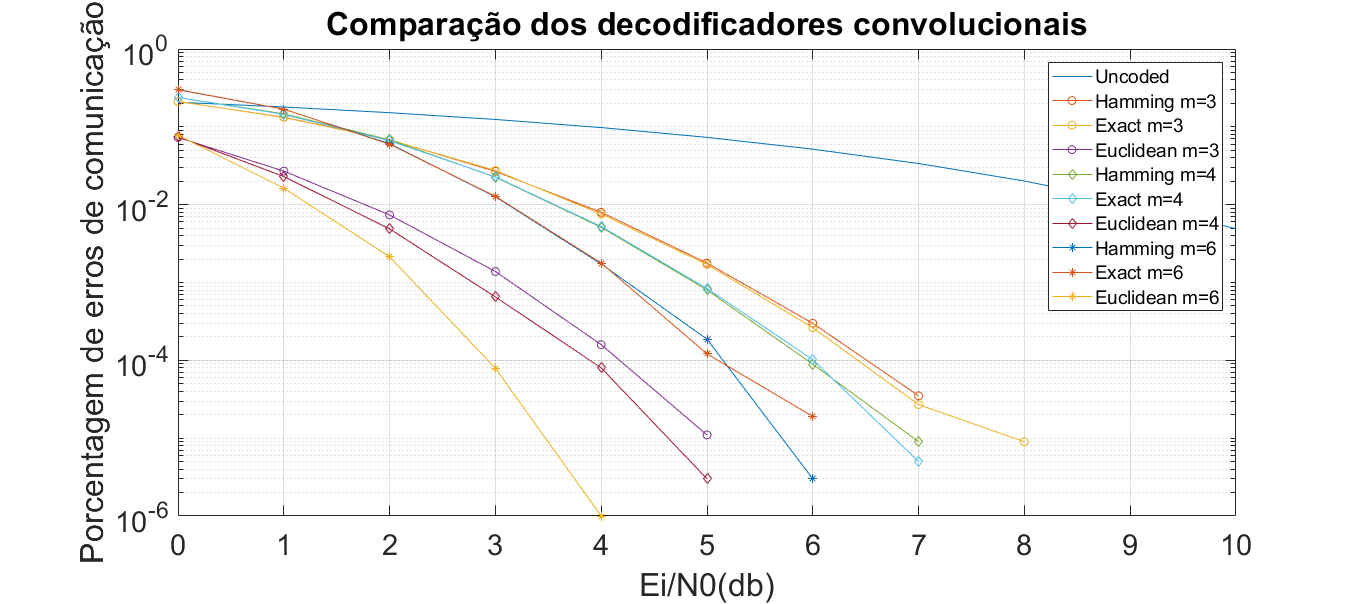
\includegraphics[width=9cm]{Fig2M}
	\captionsetup{font=scriptsize}
	\caption{Gráfico da porcentagem de erro pela razão sinal ruído normalizada para todos os valores de m\label{fig:Fig2M}}
\end{figure}

Analisando a Figura \ref{fig:Fig2M}, percebe-se que quanto maior a quantidade de memórias da máquina de estados, melhor é o desempenho do decodificador. A melhora acontece para as três métricas de cálculo de custo.

\subsection{Comparação com vários decodificadores}

Utilizando os códigos desenvolvidos em relatórios anteriores, comparou-se na Figura \ref{fig:Fig3M} o desempenho dos códigos de convolução com os de bloco e cíclicos. Para os códigos de bloco, foram testados o código de Hamming e o código desenvolvido pelo grupo. Já para os códigos cíclicos, foram testados um código BCH  e apenas os que possuíam distância mínima de Hamming suficiente para corrigir um bit: $(7,12)$ e $(8,14)$, em que o par ordenado é composto pelos bits de informação e pelo tamanho de palavra código.

\begin{figure}[H]
	\centering
	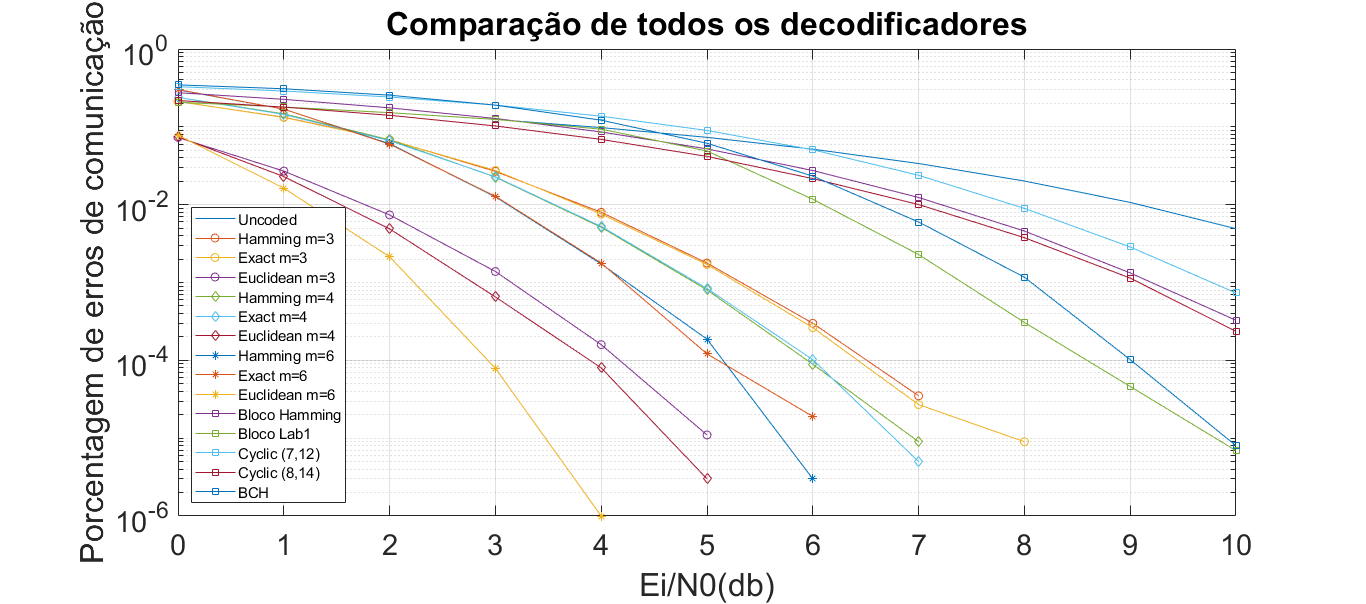
\includegraphics[width=9cm]{Fig3M}
	\captionsetup{font=scriptsize}
	\caption{Gráfico da porcentagem de erro pela razão sinal ruído normalizada para todos os decodificadores\label{fig:Fig3M}}
\end{figure}

Analisando a Figura \ref{fig:Fig3M}, percebe-se que os códigos que obtém melhor desempenho são os códigos convolucionais. Em seguida, observa-se que os códigos cíclicos possuem um desempenho, em média, melhor que os códigos de bloco, mas todos piores que os códigos convolucionais implementados.